\chapter{Fundamentação Teórica}

Texto texto texto texto texto texto texto texto texto texto texto texto texto texto texto texto texto texto texto texto texto texto texto texto texto texto texto texto texto texto texto texto texto texto texto texto texto texto texto.

\section{Subtítulo Secundário 1}

Texto texto texto texto texto texto texto texto texto texto texto texto texto texto texto texto texto texto texto texto texto texto texto texto texto texto texto texto texto texto texto texto texto texto texto texto texto texto texto, como mostra o Quadro \ref{quadro1}.


\begin{quadro}[h]
\centering

\caption{Tipos de energia analisados}
\begin{tabular}{|c|c|}
\hline
\textbf{Ano} & \textbf{Tipos de energia} \\ \hline
2017         & Mecânica                  \\ \hline
2018         & Térmica                   \\ \hline
2019         & Elétrica                  \\ \hline
2020         & Química                   \\ \hline
2021         & Atômica                   \\ \hline
\end{tabular}
\label{quadro1}
\\
\small{Fonte: Elaboração própria (2021).} 
\end{quadro}

\section{Subtítulo Secundário 2}

As citações diretas com menos de três linhas “devem estar entre aspas e devem mostrar entre parênteses o ano e a página da obra consultada.” (AUTOR, ano, página). Já as citações com mais de três linhas devem ser recuadas da margem esquerda em 4 cm, tamanho da fonte 10, espaçamento simples e texto sem aspas (ABNT, 2002, p. 2).



 \begin{citacao}
            \begin{alineas}[leftmargin=\leftskip+\labelwidth-\labelsep]
                Texto texto texto texto texto texto texto texto. Texto texto texto texto texto texto. Texto texto texto texto texto texto texto texto texto. Texto texto texto texto texto texto Texto texto texto texto texto texto. Texto texto texto texto texto texto. (\citeauthor{ref:ibmm}, \citeyear{ref:ibmm}, p. 20).
            \end{alineas}
\end{citacao}



\subsection{Subtítulo Terciário}

Texto texto texto texto texto texto texto texto texto texto texto texto texto texto texto texto texto texto texto texto texto texto texto texto texto texto texto texto texto texto texto texto texto.


\subsubsection{Subtítulo Quaternário}

Texto texto texto texto texto texto texto texto texto texto texto texto texto texto texto texto texto texto texto texto texto texto texto texto texto texto texto texto texto texto texto texto texto  (conforme exposto na Figura \ref{fig:motor}).



    \begin{figure}[H]
    	\centering
    	\caption{Motor Weg W22}
    	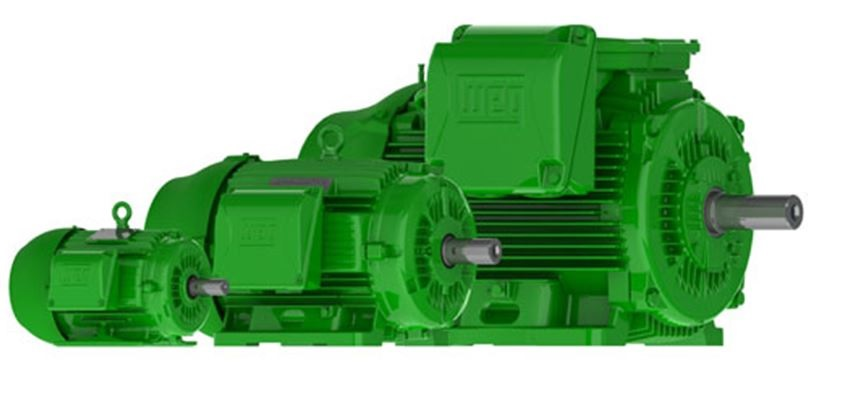
\includegraphics[scale=0.45]{figuras/motor.jpg}
    	\label{fig:motor}
    	\\
        \vspace{-0.8cm}\hspace{-7cm}\small{Fonte: WEG (2014).} 
    \end{figure}
    
    Texto texto texto texto texto texto texto texto texto texto texto texto texto texto texto conforme indica a Tabela \ref{tabela1}.

    

\begin{table}[h]
\centering
\caption{Produção de petróleo na Bahia}
\begin{tabular}{ c c }
\ChangeRT{2pt}
Ano  & Produção (1000 t) \\ \ChangeRT{2pt}
1996 & 2.536             \\ 
1997 & 2.665             \\ 
1998 & 3.056             \\ 
1999 & 3.567             \\ 
2021 & Atômica           \\ \ChangeRT{2pt}
\end{tabular}
\label{tabela1}
\\
\small{Fonte: Adaptado de ANP (2000).} 
\end{table}



    
    Texto texto texto texto texto texto texto texto texto texto texto texto texto texto texto texto texto texto texto texto texto texto texto texto texto texto texto texto texto texto texto texto texto 
    Texto texto texto texto texto texto texto texto texto texto texto texto texto texto texto texto texto texto texto texto texto texto texto texto texto texto texto texto texto texto texto texto texto como evidencia a Figura  \ref{fig:diagrama}.
    
    
    
    \begin{figure}[H]
    	\centering
    	\caption{Diagrama Fasorial}
    	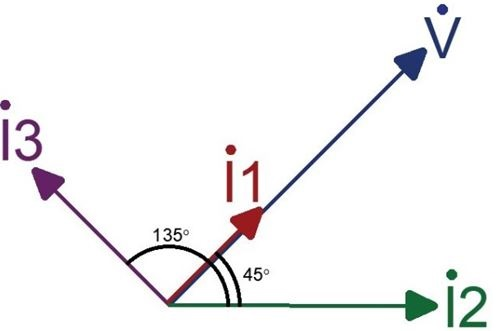
\includegraphics[scale=0.45]{figuras/diagrama.jpg}
    	\label{fig:diagrama}
    	\\
    	\vspace{0.2cm}\hspace{-3cm}\small{Fonte: Silva (2020).}
    \end{figure}
    
    Texto texto texto texto texto texto texto texto texto texto texto texto texto texto texto texto texto texto texto texto texto texto texto texto texto texto texto texto texto texto texto texto, conforme mostra a Equação \ref{eq:baskara}.
    
\begin{equation} \label{eq:baskara}
  x=\frac{-b\pm\sqrt{b^2-4ac}}{2a}
\end{equation} 
